%%%%%%%%%%%%%%%%%%%%%%%%%%%%%%%%%%%%%%%%%%%%%%%%%%%%%%%%%%%%%%%%%%%%%%%%%%%%%%%%
%2345678901234567890123456789012345678901234567890123456789012345678901234567890
%        1         2         3         4         5         6         7         8

\documentclass[letterpaper, 10 pt, conference]{ieeeconf}  % Comment this line out if you need a4paper

%\documentclass[a4paper, 10pt, conference]{ieeeconf}      % Use this line for a4 paper

\IEEEoverridecommandlockouts                              % This command is only needed if
                                                          % you want to use the \thanks command

\overrideIEEEmargins                                      % Needed to meet printer requirements.

% See the \addtolength command later in the file to balance the column lengths
% on the last page of the document
\usepackage{amsfonts}
% The following packages can be found on http:\\www.ctan.org
\usepackage{graphics} % for pdf, bitmapped graphics files
\usepackage{multirow} % for tables
%\usepackage{cite} % for bibliography with biblatex
\usepackage{braket}
\usepackage{amsfonts}
\usepackage{amsmath}
\usepackage{amssymb}
\usepackage{breqn}
\usepackage[utf8]{inputenc}
\usepackage[style=ieee,doi=false,isbn=false,url=false,date=year,minbibnames=15,maxbibnames=15,backend=biber]{biblatex}
%\renewcommand*{\bibfont}{\footnotesize}		%% Use this for papers
\setlength{\biblabelsep}{\labelsep}
\bibliography{bibRiskPaper}
%\usepackage{subfig}
%\usepackage{amsthm}
%\usepackage{mathrsfs}
\usepackage{epsfig} % for postscript graphics files
\usepackage{nomencl}
%\usepackage{mathptmx} % assumes new font selection scheme installed
\usepackage{times} % assumes new font selection scheme installed
%\usepackage{amsmath} % assumes amsmath package installed
%\usepackage{amssymb}  % assumes amsmath package installed
\graphicspath{ {figures/} }
\usepackage[capitalize]{cleveref}
\usepackage{color}
\usepackage{units}
%\usepackage[English]{babel}             %% language support
\newtheorem{definition}{Definition}
\newtheorem{assumption}{Assumption}

% Tikz stuff
\usepackage{pgfplots}                           %% support for TikZ figures
\pgfplotsset{compat=1.16}
\usepgfplotslibrary{groupplots}
\newlength{\figurewidth}
\newlength{\figureheight}

% Self defined commands
\newcommand*{\ud}{\mathrm{\,d}}

% Table stuff
\usepackage{booktabs}
\setlength{\heavyrulewidth}{0.1em}
\newcommand{\otoprule}{\midrule[\heavyrulewidth]}

\title{\LARGE \bf
A Method for Scenario Risk Quantification for Automated Driving Systems
}


\author{Arash Khabbaz Saberi, Erwin de Gelder, Hala Elrofai}
%\thanks{*This research has received funding from the European Unions Horizon 2020 research and innovation programme under ROADART Grant Agreement No 636565.}% <-this % stops a space
%\thanks{$^{1}$E. van Nunen is with the Department of Integrated Vehicle Safety, TNO, P.O.
%Box 756, 5700 AT Helmond, The Netherlands, and also with the Department of Mechanical Engineering, Eindhoven University of Technology, 5600 MB Eindhoven, The Netherlands


\begin{document}



\maketitle
\thispagestyle{empty}
\pagestyle{empty}


%%%%%%%%%%%%%%%%%%%%%%%%%%%%%%%%%%%%%%%%%%%%%%%%%%%%%%%%%%%%%%%%%%%%%%%%%%%%%%%%
\begin{abstract}
	
	
% Guideline: Context [DONE], Objective [DONE], Method, Results [DONE], Disccusion/limitations, Conclusion [DONE]. 

% Required by the ESV conference: Research Question/Objective [DONE], Methods and Data Sources, Results [DONE], Discussion and Limitations, Conclusion and relevance to session submitted 

% Left open: Method, Data Sources, Disussion and limitation, relevance. 

%TODO: Determine which track we want to go for
% Tuesday Afternoon Track C: Crash Avoidance: Automated Driving Systems (ADS) Levels 3, 4 and 5: Product Evolution; Evaluation; and Real-World Deployment Challenges
	
% Introduction
New developments in the automotive industry towards higher levels of automation are introducing new safety concerns for vehicles. Test procedure and performance measures need to be adapted for evaluation of vehicles with Automated Driving Systems (ADS). The safety and reliability of the AD vehicles must be validated in principle for all possible traffic situations/scenarios that ADS may encounter on the road, before these systems can be taken into production.

%test-driving with autonomous car prototypes on regular roads. This is a very expensive and time consuming alternative. Millions of driving kilometers are needed to get sufficient ‘driving events’ that trigger the ADS functionality under test
%The main challenge is to over-come the dilemma of testing the entire complexity of real-world traffic without the need of test-driving millions of kilometers.
%Test procedures and assessment of automotive technology to ensure implementation of new safety and comfort AD systems and functionalities has become state of the art in the last decades.
Scenario-based safety validation for automated driving is one of the proposed approach that is broadly supported by the automotive community. This is reflected in a draft standard of NHTSA and the ISO 26262 working group on SOTIF. Related projects in Germany (Pegasus [ref]) and EU (ENABLE-S3 [ref]) strongly support this approach.
%With the increasing level of automation, the vehicle needs to operate safely in a large number of different scenarios. 
%To assure the operational safety, the automated driving systems need to be assessed for this large number of scenarios. To prioritize the scenarios, risk assessment methods are required to estimate the associated risk for each scenario.
Main challenge for this approach is prioritization and selection of scenarios for testing and validation, hence risk assessment methods are required to estimate the associated risk for each scenario.

The ISO 26262:2018 [1] captures the State of the art in automotive functional safety. It defines the safety lifecycle and the related safety activities such as Hazard Identification and Risk Assessment.

 It defines risk as:
\begin{definition}
	``combination of the probability of occurrence of harm and the severity of that harm.'' 
\end{definition}

This standard gives guidelines to assess risk based on vehicle level hazardous events. A hazardous event is the combination of a vehicle level hazard with operational situation or scenario. It requires analyzing each hazardous event risk individually based on three parameters of Severity, Probability of exposure, and Comparability. The combination of these parameters contributes to constructing the Automotive Safety Integrity Level (ASIL). In this framework, each parameter is quantified in three or four levels that construct the ASIL ranking A, B, C, D, and QM. Where ASIL A represents the least critical level and in ascending order, ASIL D the most critical level. Quality Management (QM) means that the identified hazard is not critical enough for the safety processes, and the quality management system of the manufacturer should suffice for reducing the risk. We depict the ASIL ranking graph in \cref{Fig:ASILGraph}. 

\begin{figure}
	\centering
	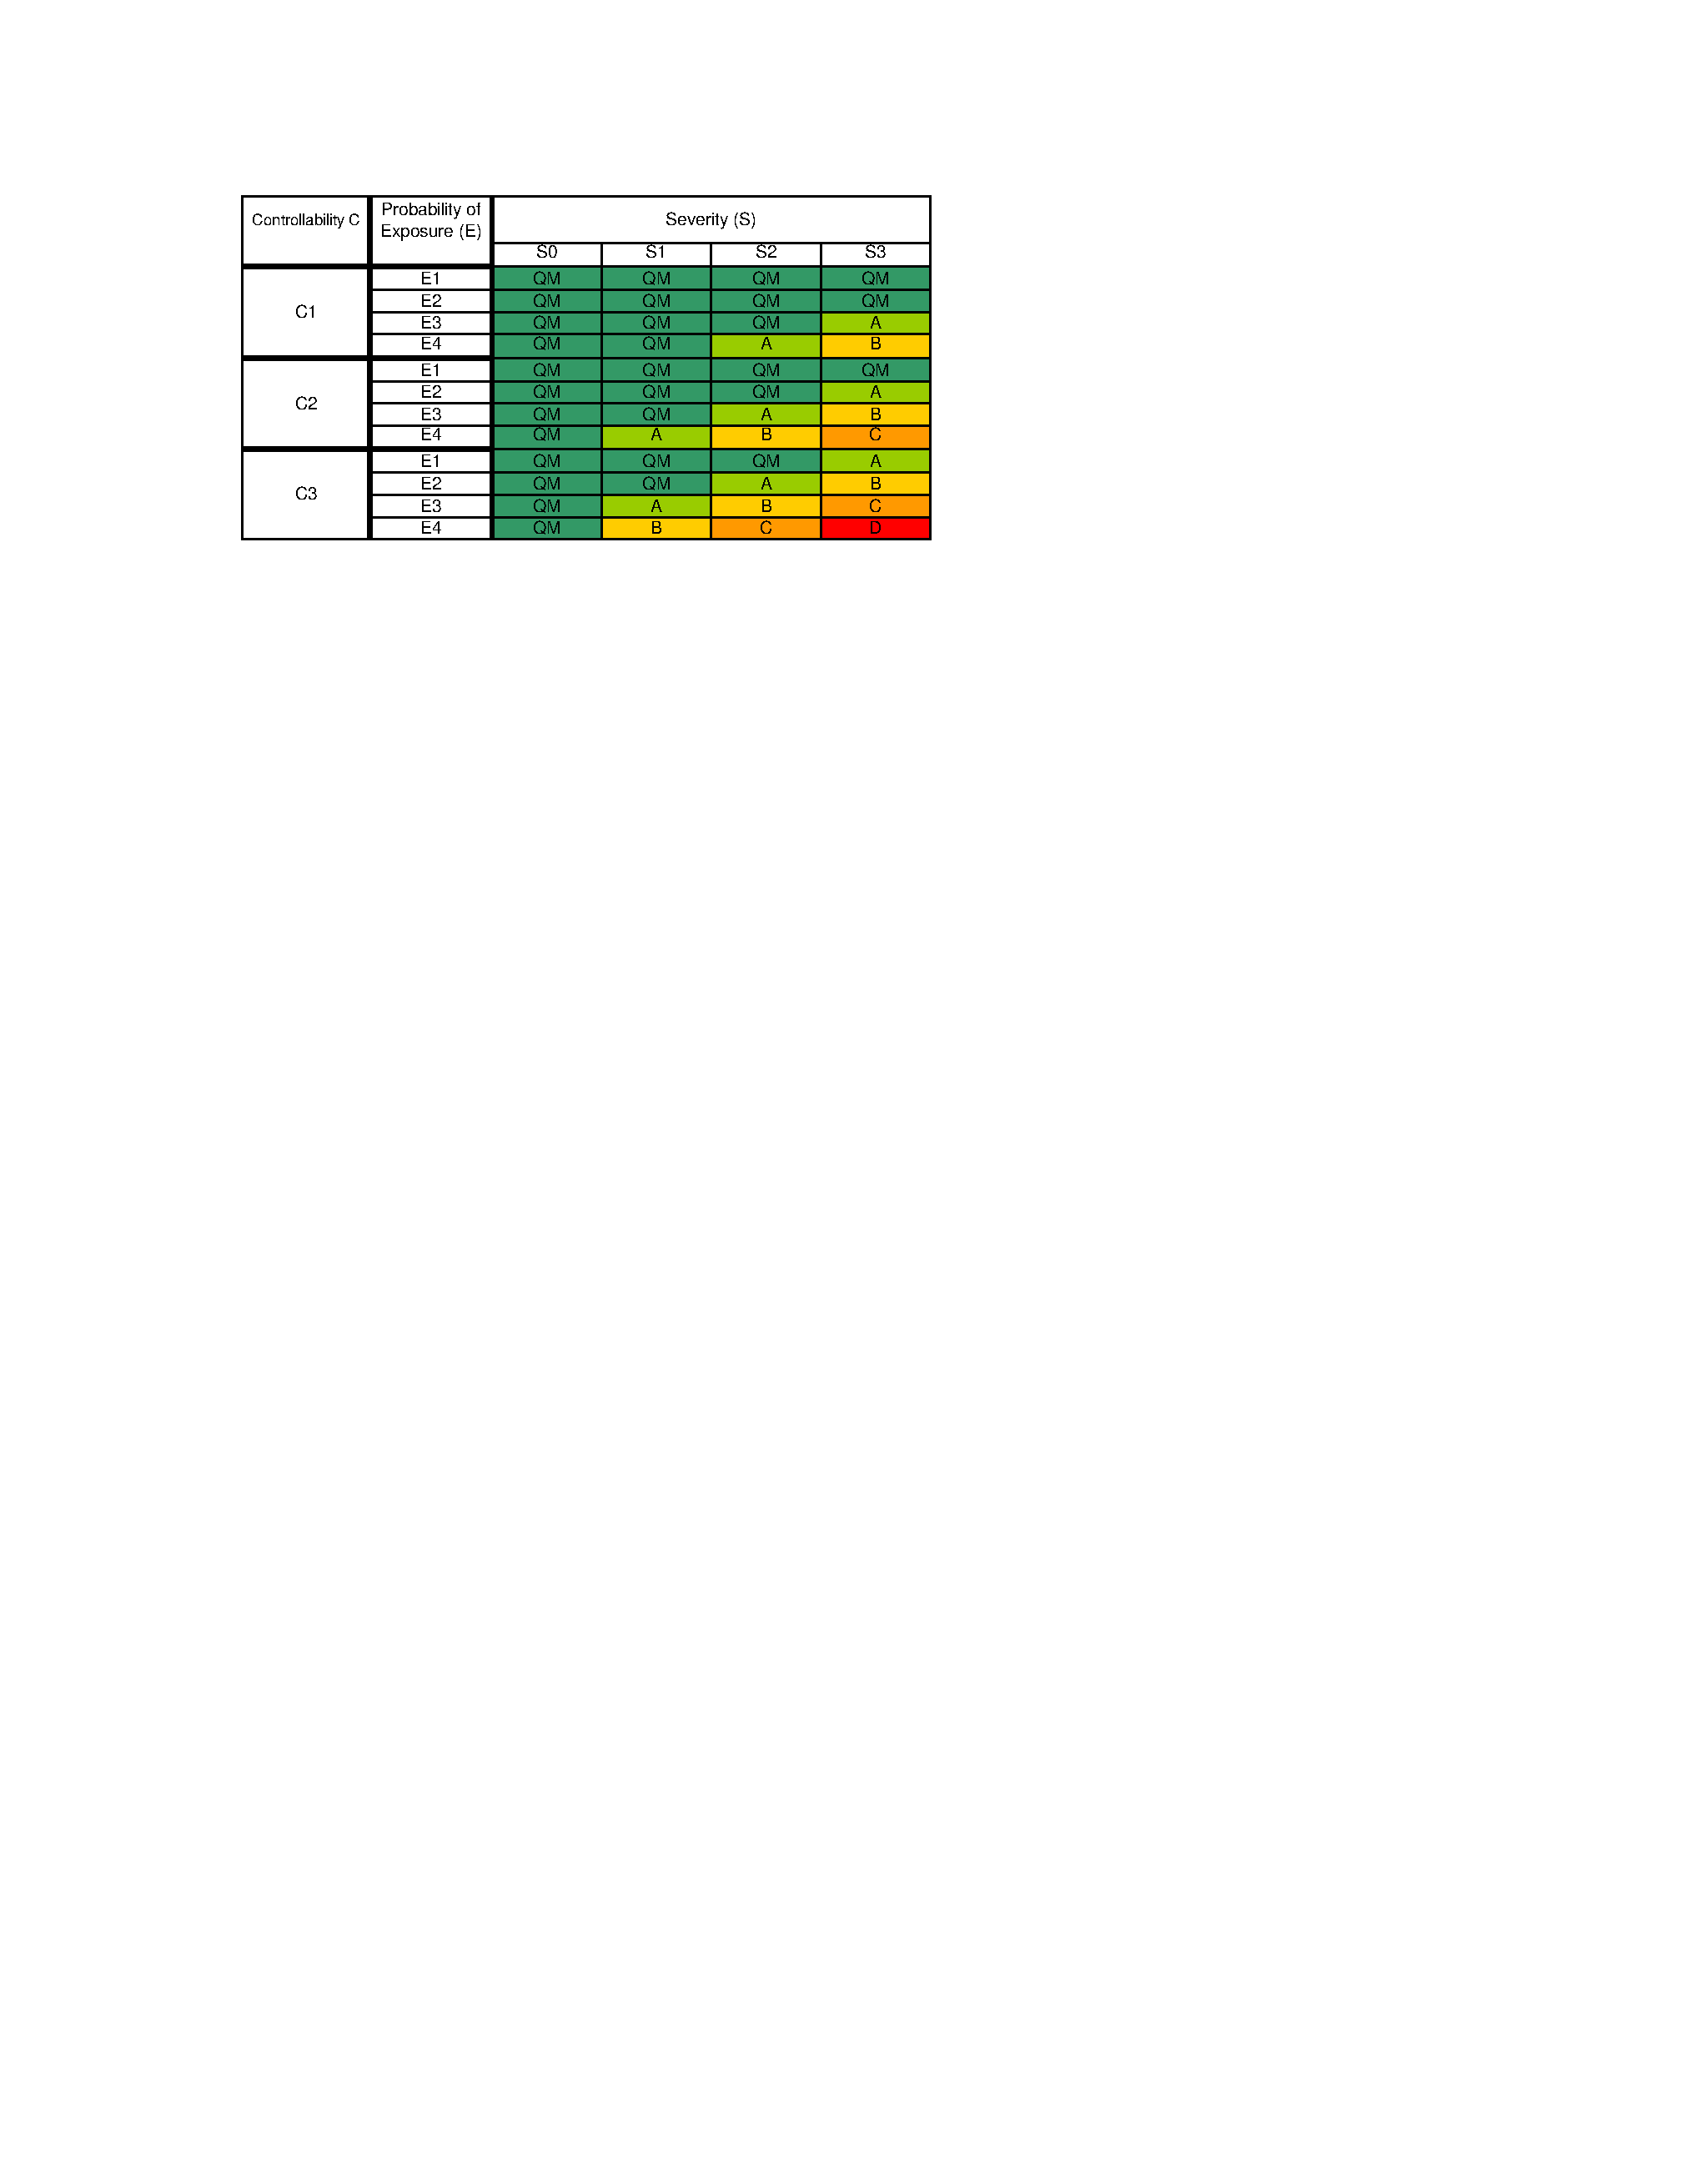
\includegraphics[width=0.9\linewidth]{./figures/ASIL}
	\caption{ASIL Risk Assessment Graph.}
	\label{Fig:ASILGraph}
\end{figure}

The ASIL methodology for risk assessment relies on the experts’ judgments of the three risk parameters. The ISO 26262 provides some general guidelines for assessing these parameters. However, the assessment is for the most part subjective and dependent on the experts who carry it out. 

%\color{red}
%Problem detention?
%The state of the art risk assessment methods in the automotive domain, such as the Hazard Analysis and Risk Assessment (HARA) of ISO~26262:2018, have a qualitative nature and rely on expert's judgment for ranking the severity and probability of risks(ref).
%
%Moreover, these methods are only capable of evaluating the risk of a single (hazardous) event within the context of a generic operational situation.}
%\color{black}

The objective of this paper is to introduce a method for analysis and quantification of the risk of a driving scenario taking into account the entire operational situations and their interrelation. 

% Method

For the proposed method, we assume that a scenario consists of events, activities (performed by different actors), and environmental conditions.
Next, the risk of a driving scenario is considered as the product of severity of the outcome of a scenario and probability of the exposure of that scenario.
We introduce a systematic method for calculating this probability, 
	where we assume a causal relation between the activities and events that constitute a scenario. 
By making educated assumptions on the dependencies among the different activities, events, and environmental conditions, 
	we simplify the calculation of the probability of the exposure of a scenario. 
Finally, Monte Carlo simulations are employed for computing the risk of a scenario.


% Results
To illustrate the use of the proposed method, 
	we perform a case study by applying our proposed method for risk analysis of a cut-in scenario.	
We use naturalistic driving data acquired from field studies on the Dutch highways to determine the likelihoods of the events, activities, and environmental conditions that constitute the cut-in scenarios. Monte Carlo simulations are employed for determining the outcome of the cut-in scenarios, e.g., a collision or a near miss, given a state-of-the-art highway pilot system. 

% Discussion and limitations
The presented case study illustrates the potential of the proposed risk estimation method. The main limitation of the presented case study is the limited amount of data used. Furthermore, we applied the proposed method for only one type of driving scenario, while the full potential can be better demonstrated by applying the method to a wider range of scenarios.

% Conclusion
Using our proposed method, we can compare the safety criticality of various scenarios in a quantitative manner, which can be used as a safety metric for evaluating automated driving systems. 
This can lead to stronger justification for design decisions and test coverage for developing automated vehicle functionalities. 


%% No need to mention the challenges in the abstract
%%% Arash: This is required from the ESV to discuss the limitations. I think it's beacause this is more like an extended asbtact. 
% The challenge for applying this method is gathering enough data for quantification of scenario activities.
\end{abstract}


%%%%%%%%%%%%%%%%%%%%%%%%%%%%%%%%%%%%%%%%%%%%%%%%%%%%%%%%%%%%%%%%%%%%%%%%%%%%%%%%

\section{Introduction}
\label{sec:introduction}

TODO

\color{red}
For Arash and Hala: please use \\{\tt \textbackslash cref\{sec:introduction\}}\\ to refer to sections, figures etc. It automatically adds things as `Section': e.g., \cref{sec:introduction}.
\color{black}

The introduction contains: 
\begin{itemize}
	\item Setting up the context of automated driving
	\item Giving some background information about the hazard analysis and risk assessment in the ISO~26262 standard
	\item The gap (the problem) We currently have this as a separate chapter, we could move it to introduction depending on the length. 
	\item our contribution. 
	\item paper structure
\end{itemize}
\section{Problem definitions}
\label{sec:problem} % Arash

This Section presents: 
\begin{itemize}
	\item Why risk assessment matters?
	\item What is currently the risk estimation method? 
	\item What is lacking in this approach? 
	\item What need to be done more? 
\end{itemize}

In this section we position our research in the automotive safety engineering domain. 
We present the current risk assessment methods and discuss their limitation and the impact of these limits.
The argue that advancement in the risk assessment methods are required for achieving higher levels of automation in the automotive domain. 

\subsection{Why risk assessment?}

Safety means avoiding risk. 
The risk associated with driving may come from multiple sources. 
It could be a traffic situation in which a sequence of uncorrelated actions performed by different actors lead to an accident. 
The risk could also be due to technical failure originating from a system fault. 
%This type of faults and failures should be avoided by the manufacturers of the automotive systems (OEMs and Tiers), 
%	while the later is a responsibility of the traffic participants. 
For the former, the manufacturers are deemed responsible; 
	therefore, they put a lot of effort on the quality  assurance of their products 
		and for understanding and mitigating technical safety issues.  
The later comes into the public domain and road authorities are responsible for minimizing the risk by good design of roads and traffic rules. 
The  risk, however, cannot be avoided fully. 
There is always a certain amount of \textit{residual risk} remaining after taking risk avoidance/mitigation measures. 

Understanding the risk and measuring it is crucial in both directing the effort on avoiding or mitigating the impacts. 
Moreover, formulating and opinion about when using a system is ``safe enough'' depends on the ability to measure the risk. 
	

\subsection{Risk assessment in ISO~26262}

Risk is defined in ISO~26262 as:
\begin{definition}
	``combination of the probability of occurrence of harm and the severity of that harm'' 
\end{definition}



Risk assessment is an integral part of the safety life-cycle of ISO~26262 and one of the earlier activities. 
During risk assessment, the identified hazardous events are analyzed and the associated severity, probability of exposure and controllability are estimated and assigned to some predefined levels. 
The combination of the estimated severity, exposure and controllability contribute to construct the Automotive Safety Integrity Level (ASIL). 


This is the domain of functional safety. 
The goal of functional safety is to avoid \emph{unreasonable} risk\footnote{Unreasonable risk is judged according to the the society's acceptance of level of risk.} that is due to some sort of malfunctioning.


\section{Nomenclature} % Erwin (use the other paper) & Arash
\label{sec:definitions}

TODO: give more examples
First, we introduce the following notions:
\begin{enumerate}
\item Risk = Severity $\times$ Probability
\item Severity: a quantitative measure, depending on the impact velocity.
\item Condition:
\item Actor: the relevant actors here are the lead vehicle (denoted with L), the following vehicle (F) and the communication unit (V2V)
\item Activity: the relevant actions here are braking, and failure.
\item Scenario:
\end{enumerate}

\section{Proposed Risk Estimation Method}
\label{sec:method}
 
In the Hazard Analysis and Risk Assessment (HARA) required by the ISO~26262 standard, the estimation of Automotive Safety Integrity Level (ASIL) is calculated based on a so-called single specific hazardous event \cite{ISO26262}.
Although the operational situation in which this single event occurs as well as the operating mode are considered in the analysis, still the proceeding and successive events are not taken into account.
In this paper, we propose a new method to estimate the risk of a certain scenario considering the whole chain of activities and conditions that constitute the scenario.
The estimated risk is based on real-world driving data. To estimate the risk, we will quantify the exposure and the severity. In \cref{Tab:Terms}, we present the definitions of the terms that are used in our proposed methodology. 

\begin{table}
	\centering
	\caption{The terms and definitions}
	\label{Tab:Terms}
	\begin{tabular}{p{0.15\linewidth} p{0.75\linewidth}} \hline
		\textbf{Term} & \textbf{Definition} \\ \hline
		Severity & An estimate of the extent of harm to one or more individuals that can occur in a potentially hazardous event~\cite{ISO26262} \\
		Exposure & The state of being in a driving scenario \\
		Risk & The combination of the probability of occurrence of harm and the severity of that harm~\cite{ISO26262} \\ 
		Condition & The constant parameters describing the environmental aspects of the operational design domain\footnote{``Operating conditions under which a given driving automation system or feature thereof is specifically designed to function'' \cite{sea2018j3016}.} \\
		Actor & An element of a scenario acting on its own behalf~\cite{ulbrich2015} \\ 
		Scenario & A quantitative description of the activities of the ego vehicle and other actors and the conditions from the static environment \\ \hline
	\end{tabular}
\end{table}

As explained in \cref{Tab:Terms}, a scenario consist of a set of conditions and activities, denoted by $A$ and $C$, respectively. We formulate the exposure as the average number of occurrences of the activities $A$ under the conditions $C$, denoted by $\lambda_{A,C}$. The severity is the likelihood of the potential hazardous consequence $R$ given the activities $A$ and the conditions $C$, denoted by the conditional probability $P(R|A,C)$. The risk is computed as the multiplication of the exposure and the severity. 

The proposed method is summarized in \cref{fig:method}. To compute the exposure, we calculate the likelihood of the conditions, denoted by $P(C)$, and the conditional likelihood of the activities, denoted by $P(A|C)$, based on real-world driving data. This is explained in detail in \cref{sec:exposure}. For the estimation of the severity, we consider all possible scenarios that are subject to a set of conditions $C$ and consist of the activities $A$. Therefore, we parametrize the scenarios using the parameter vector $\theta$. Based on the real-world driving data, the probability density function of the parameters $P(\theta|A,C)$ is estimated. Next, using simulations, we estimate $P(R|\theta,A,C)$, the likelihood of a potential hazardous consequence $R$ given a parametrized scenario. The details of the estimation of the severity are presented in \cref{sec:severity}. Finally, in \cref{sec:risk}, we describe how the risk is estimated based on the estimated exposure and severity.

\begin{figure}
	\centering
	\includestandalone[width=\linewidth]{figures/method}
	\caption{Proposed method for quantifying the risk. The risk is a multiplication of the exposure and the severity, explained in \cref{sec:exposure,sec:severity}, respectively.}
	\label{fig:method}
\end{figure}

%The following steps are followed when computing the risk:
%\begin{enumerate}
%	\item Estimate the likelihood of the conditions $P(C)$.
%	\item Estimate the exposure $\lambda_{A,C}$.
%	\item Parametrize the scenario with a parameter vector $\theta$.
%	\item Estimate the distribution of $\theta$ for this scenario class, i.e., $P(\theta|A,C)$.
%	\item Use simulations to estimate the severity, i.e., $P(R|A,C)$.
%	\item Compute the risk of a scenario class denoted by $\lambda$.
%	\item Compute the number of hours that can be driven without any harm associated with the given scenario class.
%\end{enumerate}


\subsection{Calculate exposure}
\label{sec:exposure}

The scenarios are subject to $n_C$ conditions, denoted by $C_1, \ldots, C_m$. For the sake of brevity, all conditions together are denoted by $C$, i.e., $P(C_1, \ldots, C_{n_C})=P(C)$. Many of these conditions might be based on the operational design domain of the AD system and might include conditions with respect to the infrastructure, weather conditions, lighting conditions, and geographical locations. 

The first step is to compute the joint probability of the conditions, i.e., $P(C)$. In case these conditions are independent, the probability can be computed by simply multiplying the individual likelihoods for each condition, i.e., $P(C)=P(C_1)\cdot\ldots\cdot P(C_{n_C})$. This, however, might not necessarily be the case, which requires either to compute the joint probability or to compute conditional probabilities. In some cases, it might also be reasonable to simply assume that the likelihood of certain conditions are independent.

Note that the the defined conditions might not be the same as the conditions under which the data is collected that is used to compute $P(C)$. This might require additional assumptions, see our example in \cref{sec:example exposure}.

To calculate the exposure, the average number of occurrences of the activities that constitute the scenarios that fall into the specified scenario class within a certain time interval need to be estimated. Let $n_A$ denote the number of activities, such that $A_1, \ldots, A_{n_A}$ denote the activities. For the sake of brevity, all activities together are denoted by $A$. 

Without loss of generality, we assume that the time interval is an hour. To estimate the number occurrences of the activities, the data for which the conditions $C$ are satisfied are analyzed. The average number of occurrences of the activities $A$ for each hour of driving for which the conditions $C$ are satisfied is denoted by $\lambda_{A|C}$. Next, we can calculate the average number of occurrences of the activities $A$ under the conditions $C$ for each hour of driving:
\begin{equation}
	\lambda_{A,C} = \lambda_{A|C} \cdot P(C).
\end{equation}

Regarding the scenarios that fall into the specified scenario class, we assume the following:
\begin{itemize}
	\item The occurrence of one scenario consisting of activities $A$ and conditions $C$ does not affect the probability that a second scenario consisting of activities $A$ and conditions $C$ occurs.
	\item The rate at which a scenario consisting of activities $A$ and conditions $C$ occurs is constant. I.e., $\lambda_{A,C}$ is constant.
	\item Two scenarios consisting of activities $A$ and conditions $C$ cannot occur at exactly the same time instant.
\end{itemize}
Based on these assumptions, the number of occurrences of scenarios consisting of activities $A$ and conditions $C$ is distributed according to the Poisson distribution:
\begin{equation}
	P(k\text{ times }A,C\text{ in an hour}) = \exp \left\{-\lambda_{A,C} \right\} \frac{\lambda_{A,C}^k}{k!}.
\end{equation}



\subsection{Severity}
\label{sec:severity}

The first step towards estimating the severity is to parametrize the scenarios with a parameter vector $\theta \in \mathbb{R}^d$. The parametrization enables the generation of infinitely many unique individual test cases that resemble the scenarios found in naturalistic driving \cite{deGelder2017assessment,elrofai2018scenario}.

In case the parameters are dependent, which is often the case, it is important that the number of parameters is limited to avoid the curse of dimensionality \cite{scott2015multivariate}. This often requires some assumptions. An example is presented in \cref{sec:example severity}.

To estimate the probability density function (pdf) of the parameter vector $\theta$, i.e., $P(\theta|A,C)$, either parametric models, non-parametric models, or a combination of the two can be used. In case of parametric models, a certain functional form of the pdf is assumed. For example, it might be assumed that the pdf can be modeled using a Gaussian distribution. In this paper, we present a non-parametric approach using Kernel Density Estimation (KDE) \cite{rosenblatt1956remarks, parzen1962estimation}. Using KDE, there is no assumption on the functional form of the pdf because the shape of the pdf is automatically computed.

Using KDE, the estimated pdf is given by
\begin{equation}
	\label{eq:kde}
	P(\theta|A,C) = \frac{1}{nh^d} \sum_{i=1}^n K\left(\frac{\theta - \theta_i}{h}\right).
\end{equation}
Here, $K(\cdot)$ is an appropriate kernel function and $h$ denotes the bandwidth. From the data, $n$ scenarios are extracted and each scenario is parametrized with $\theta_i$. The choice of the kernel $K(\cdot)$ is not as important as the choice of the bandwidth $h$ \cite{turlach1993bandwidthselection}. Often, a Gaussian kernel is used, which is given by
\begin{equation}
	\label{eq:gaussian kernel}
	K(u) = \frac{1}{\left( 2\pi \right)^{d/2}} \exp \left\{ -\frac{1}{2} \|u\|^2 \right\},
\end{equation}
where $\|u\|^2$ denotes the squared 2-norm of $u$, i.e., $u^T u$.

The bandwidth $h$ controls the amount of smoothing. For the kernel of \cref{eq:gaussian kernel}, the same amount of smoothing is applied in every direction, although this can easily be extended to a multi-dimensional bandwidth, see, e.g., \cite{scott2005multidimensional, chen2017tutorial}. There are many different ways of estimating the bandwidth, ranging from simple reference rules like, e.g., Scott's rule of thumb \cite{scott2015multivariate} or Silverman's rule of thumb \cite{silverman1986density} to more elaborate methods; see \cite{turlach1993bandwidthselection, bashtannyk2001bandwidth, jones1996brief, chiu1996comparative} for reviews of different bandwidth selection methods. 

Let $R$ denote a potential hazardous consequence of a scenario. We define the severity of a scenario with activities $A$ and conditions $C$ as the probability of $R$, given the activities $A$ and $C$, i.e., $P(R|A,C)$. We cannot evaluate $P(R|A,C)$ directly, because the outcome of a scenario highly depends on the parametrization $\theta$. Therefore, we estimate $P(R|\theta,A,C)$ through a simulation of the scenario with parameters $\theta$. Using $P(\theta|A,C)$ from \cref{eq:kde}, we can compute 
\begin{equation} \label{eq:probability R theta}
	P(R,\theta|A,C) = P(R|\theta,A,C) \cdot P(\theta|A,C).
\end{equation}
To obtain $P(R|A,C)$, we need to integrate \cref{eq:probability R theta} over $\theta$, i.e., 
\begin{equation} \label{eq:probability R}
	P(R|A,C) = \int_{\mathbb{R}^d} P(R|\theta,A,C) \cdot P(\theta|A,C) \ud \theta.
\end{equation}

One approach to evaluate the integral of \cref{eq:probability R} is to perform Monte Carlo simulations. For sufficiently large $N$, we have
\begin{equation} \label{eq:monte carlo}
	P(R|A,C) \approx \frac{1}{N} \sum_{k=1}^N P(R|\theta_k,A,C), \, \theta_k \sim P(\theta|A,C).
\end{equation}

To improve the accuracy of \cref{eq:monte carlo}, importance sampling can be used where the parameters $\theta$ are drawn from another distribution with a focus on the critical scenarios, see, e.g., \cite{deGelder2017assessment}.



\subsection{Calculating the risk}
\label{sec:risk}

Analogous to the exposure, we define the risk as the number of occurrences of the harmful outcome $R$ in a scenario consisting of activities $A$ and conditions $C$ in a certain time interval. Let $\lambda$ denote the average number of these occurrences in an hour of driving. The chain rule of probability tells us that this equals the sum of $\lambda_{A,C}$ (i.e., the exposure) and $P(R|A,C)$ (i.e., the severity):
\begin{equation} \label{eq:risk}
	\lambda = \lambda_{A,C} \cdot P(R|A,C)
\end{equation}

Analogous to the number of occurrences of a scenario consisting of activities $A$ and conditions $C$, we assume that the number of occurrences of a harmful outcome $R$ in a scenario consisting of activities $A$ and conditions $C$ can be modeled using a Poisson distribution:
\begin{equation} \label{eq:poisson risk}
	P(k\text{ times }R,A,C\text{ in an hour}) = \exp \left\{ -\lambda \right\} \frac{\lambda^k}{k!}.
\end{equation}

Using \cref{eq:poisson risk}, to calculate the probability of not having the harmful outcome $R$ in a scenario consisting of activities $A$ and conditions $C$ we simply need to use $k=0$:
\begin{equation} \label{eq:no harm}
	P(\text{no }R,A,C\text{ in one hour}) = \exp \left\{ -\lambda \right\}.
\end{equation}


%Let $E$ be the final event that might result in a risky situation/harm. The probability $P$ of the exposure of a harm/risk in a certain scenario is then given by 
%\begin{equation}
%P(E,A_1,A_2,...A_n,C_1,C_2,..,C_m)=P(E,A,C) \label{eq:secM1}
%\end{equation}
%where $n$ is the number of performed activities within the scenario and $m$ is the number of conditions in the same scenario.
%Since the harm event $E$ depends on the performed actives and scenario conditions, to compute \ref{eq3} requires computing $P(A,C)$ first.
%\begin{equation}
%P(A,C)=P(A|C) \cdot P(C) \label{eq:secM2}
%\end{equation}

\section{Case Study} % Erwin & Hala
%\label{sec:example}

In this section, we present a case study to illustrate the method of quantifying the risk for a cut-in scenario. We will first describe the cut-in scenario and the use case. The actual system for which the risk is computed is presented in next. After these two steps, we will go through the steps of our proposed method.



\subsection{The cut-in scenario and the use case}
%\label{sec:scenario class}

We want to quantify the risk for cut-in scenarios that are linguistically described as follows: while the ego vehicle drives at a moderate to high speed while staying in its lane, another vehicle cuts into the lane of the ego vehicle, such that this vehicle becomes the ego vehicle's lead vehicle. Furthermore, the ego vehicle needs to brake to prevent a collision.

For the quantification of the risk, 60 hours of data (see also \cite{deGelder2017assessment}) are collected by driving a specific route in and between Eindhoven and Helmond, The Netherlands, with twenty different drivers, each driving the route twice. Therefore, it is assumed that the use case of the AD system is driving this route. We will use the data for the estimation of the risk. Hence, we will make use of the following assumption:
\begin{assumption}
	The recorded naturalistic driving data is representative for what a vehicle with the AD system might encounter along the same route.
\end{assumption}



\subsection{System-under-test}
%\label{sec:system}

To reduce efforts for the assessment, often simulations are employed. However, even simulations can consume considerable time, as these simulations might run real-time \cite{shah2018airsim} or slower when a higher level of detail is used \cite{zofka2016testing}. For our method, we will simplify the simulations, such that the total required time on a common computer is in the order of minutes. Since we are interested in approximate results, a high level of detail is not required. 

To simplify the system-under-test, it is assumed that the system's desired acceleration is similar to the adaptive cruise control defined in \cite{deGelder2017assessment}, i.e.,
\begin{equation}
	\label{eq:desired acceleration} 
	u(t) = k_{\mathrm{d}}(v(t))(d(t) - \tau_{\mathrm{h}} v(t) - s_0) + k_{\mathrm{v}}\left(\dot{d}(t) - ha(t) \right),
\end{equation}
with
\begin{equation}
	\label{eq:gain}
	k_{\mathrm{d}}(v(t)) = k_{\mathrm{d1}} + \left( k_{\mathrm{d2}} - k_{\mathrm{d1}} \right) \exp \left\{ -\frac{v(t)^2}{2\sigma_{\mathrm{d}}} \right\}.
\end{equation}
Here, $v$ is the speed of the ego vehicle, $d$ denotes the clearance between the ego vehicle and its predecessor, i.e., the vehicle that performs the cut-in. The relative speed is denoted by $\dot{d}$ and $a$ refers to the acceleration of the ego vehicle. The ego vehicle is modeled using a first order model with a time delay, i.e.,
\begin{equation}
	\label{eq:vehicle model}
	\tau \dot{a}(t) + a(t) = u(t - \theta).
\end{equation}
Furthermore, the deceleration is limited at $\unit[-6]{ms^{-2}}$. A description of the constants of \cref{eq:desired acceleration,eq:gain,eq:vehicle model} are listed in \cref{tab:constants}. The controller runs at \unit[100]{Hz}.

\begin{table}
	\centering
	\caption{The constants used for the simple automation system of \cref{eq:desired acceleration,eq:gain,eq:vehicle model}.}
	\label{tab:constants}
	\begin{tabular}{clc}
		\toprule
		Parameter & Description & Value \\ \otoprule
		$\tau_{\mathrm{h}}$ & Desired headway time & \unit[2.0]{s} \\
		$s_0$ & Safety distance & \unit[1.5]{m} \\
		$k_{\mathrm{d1}}$ & Distance gain at high speed & $\unit[0.7]{s^{-2}}$ \\
		$k_{\mathrm{d2}}$ & Distance gain at low speed & $\unit[2.0]{s^{-2}}$ \\
		$\sigma_{\mathrm{d}}$ & Shaping coefficient of distance gain & $\unit[5]{ms^{-1}}$ \\
		$k_{\mathrm{v}}$ & Speed difference gain & $\unit[0.35]{s^{-1}}$ \\
		$\tau$ & Time constant of the vehicle model & \unit[0.1]{s} \\
		$\theta$ & Delay of the vehicle response & \unit[0.2]{s} \\
		\bottomrule
	\end{tabular}
\end{table}

Note that there is no intervention of a human:
\begin{assumption}
	The ego vehicle is fully controlled by the automation system as defined by \cref{eq:desired acceleration,eq:gain}. Hence, there is no intervention of a human.
\end{assumption}



\subsection{Calculate exposure}
%\label{sec:example exposure}

The cut-in scenarios are subject to the following conditions:
\begin{itemize}
	\item $C_1$: The speed of the ego vehicle is within the range of \unit[60]{km/h} and \unit[130]{km/h}.
	\item $C_2$: There are no restrictions on the weather conditions.
	\item $C_3$: There are no restrictions on the lighting conditions.
\end{itemize}

Obviously, because there are no restrictions to the weather and lighting conditions, we have $P(C_2,C_3)=1$. For the first condition, we can use the data to estimate the likelihood. The data, however, has been recorded during sunny weather at daylight. Therefore, we need to following assumption.

\begin{assumption} \label{asm:conditions}
	Let $C_2'$ and $C_3'$ denote the conditions of having sunny weather and daylight, respectively. Then we have $P(C_1|C_2,C_3)=P(C_1|C_2',C_3')$.
\end{assumption}

From the data, it appeared that $P(C_1|C_2',C_3')=0.20$. Using \cref{asm:conditions}, we have
\begin{equation}
	P(C) = P(C_1,C_2,C_3) = P(C_1|C_2',C_3')\cdot P(C_2,C_3) = 0.20.
\end{equation}

The cut-in scenarios consist of the following activities:
\begin{itemize}
	\item $A_1$: The ego vehicle is lane following.
	\item $A_2$: The target vehicle is driving in an adjacent lane in the same direction as the ego vehicle.
	\item $A_3$: After activity $A_2$, the target vehicle performs a lane change towards the lane of the ego vehicle, such that the ego vehicle needs to brake.
	\item $A_4$: The automation system detects the cut-in.
	\item $A_5$: After activity $A_4$, the automation system activates the brakes of the ego vehicle.
\end{itemize}

The likelihood of the activities $A_1$, $A_2$, and $A_3$ can be estimated using the data. It is assumed that the ego vehicle needs to brake if the target vehicle is driving slower and the headway time is less than three seconds. In case of a slower target vehicle with a larger headway time, the scenario is referred to as a gap closing scenario \cite{semsarkazerooni2016cacc, gelder2016pacc}.

For simplicity, we assume the following:
\begin{assumption}
	The automation system always detects the cut-in and activates the brakes after detecting the cut-in, such that $P(A_4,A_5|A_1,A_2,A_3,C) = 1$.
\end{assumption}

Using this assumption, we can compute $\lambda_{A|C}$ by detecting the number of occurrences of the activities $A_1$, $A_2$, and $A_3$ under the conditions $C$. Based on the dataset, we have $\lambda_{A|C}=\unit[9.9]{h^{-1}}$, i.e., in each hour that the ego vehicle is driving in a speed range of \unit[60]{km/h} and \unit[130]{km/h}, there are on average $9.9$ cut-ins with the target vehicle driving slower than the ego vehicle, such that the headway time after the cut-in is less than three seconds. From this, it simply follows that
\begin{equation}
	\lambda_{A,C} = \lambda_{A|C} \cdot P(C) = 2.0.
\end{equation}



\subsection{Calculating severity}
%\label{sec:example severity}

To limit the number of parameters, we assume the following:
\begin{assumption}
	The ego vehicle is driving at a constant speed at the moment of the cut-in of the target vehicle, i.e., the moment that the target vehicle enters the lane of the ego vehicle.
\end{assumption}
\begin{assumption}
	The target vehicle is driving at a constant speed.
\end{assumption}
Both assumptions can be justified using the data. In case of the ego vehicle, the average acceleration at the moment of the cut-in is $\unit[-0.29]{ms^{-2}}$ and the standard deviation equals $\unit[0.50]{ms^{-2}}$. In case of the target vehicle, the average deceleration at the moment of the cut-in is $\unit[0.05]{ms^{-2}}$ and the standard deviation equals $\unit[0.37]{ms^{-2}}$. As a result, the scenario is parametrized using $d=3$ parameters:
\begin{enumerate}
	\item The clearance between the target vehicle and the ego vehicle at the moment of the cut-in, i.e., the moment than the target vehicle enters the lane of the ego vehicle.
	\item The speed of the ego vehicle at the moment of the cut-in.
	\item The speed of the target vehicle throughout the whole scenario.
\end{enumerate}


A histogram of the data of the parameters is shown in \cref{fig:histogram}. The probability density function is estimated using the KDE of \cref{eq:kde} with the Gaussian kernel of \cref{eq:gaussian kernel}. Before applying KDE, the data is scaled, such that the standard deviation equals one for each parameter. We use leave-one-out cross validation to compute the bandwidth $h$ (see also \cite{duin1976parzen}) because this minimizes the Kullback-Leibler divergence between the real underlying pdf and the estimated pdf \cite{turlach1993bandwidthselection,zambom2013review}. The resulting bandwidth equals $h=0.198$. The marginal probability distributions coming from the resulting joint distribution, i.e. the KDE, are shown in \cref{fig:histogram} by the black lines.

\setlength\figurewidth{0.5\linewidth}
\setlength\figureheight{0.25\linewidth}
\begin{figure}
	\centering
	% This file was created by matplotlib2tikz v0.6.17.
\begin{tikzpicture}

\begin{groupplot}[group style={group size=1 by 3}]
\nextgroupplot[
xlabel={Clearance [m]},
ylabel={Density},
xmin=8.12085897227673, xmax=100.239482786353,
ymin=0, ymax=0.0358233749416452,
width=\figurewidth,
height=\figureheight,
tick align=outside,
tick pos=left,
x grid style={white!69.01960784313725!black},
y grid style={white!69.01960784313725!black},
axis x line*=bottom,
axis y line*=left,
scaled y ticks = false,
y tick label style={/pgf/number format/fixed}
]
\draw[draw=black,fill=gray] (axis cs:12.3080691456438,0) rectangle (axis cs:16.4952793190109,0.0120414705686202);
\draw[draw=black,fill=gray] (axis cs:16.4952793190109,0) rectangle (axis cs:20.682489492378,0.0100345588071835);
\draw[draw=black,fill=gray] (axis cs:20.682489492378,0) rectangle (axis cs:24.8696996657451,0.0260898528986771);
\draw[draw=black,fill=gray] (axis cs:24.8696996657451,0) rectangle (axis cs:29.0569098391121,0.034117499944424);
\draw[draw=black,fill=gray] (axis cs:29.0569098391122,0) rectangle (axis cs:33.2441200124792,0.0160552940914936);
\draw[draw=black,fill=gray] (axis cs:33.2441200124792,0) rectangle (axis cs:37.4313301858463,0.0180622058529303);
\draw[draw=black,fill=gray] (axis cs:37.4313301858463,0) rectangle (axis cs:41.6185403592134,0.0220760293758037);
\draw[draw=black,fill=gray] (axis cs:41.6185403592134,0) rectangle (axis cs:45.8057505325805,0.0100345588071835);
\draw[draw=black,fill=gray] (axis cs:45.8057505325805,0) rectangle (axis cs:49.9929607059476,0.0160552940914936);
\draw[draw=black,fill=gray] (axis cs:49.9929607059476,0) rectangle (axis cs:54.1801708793146,0.0220760293758038);
\draw[draw=black,fill=gray] (axis cs:54.1801708793146,0) rectangle (axis cs:58.3673810526817,0.0120414705686202);
\draw[draw=black,fill=gray] (axis cs:58.3673810526817,0) rectangle (axis cs:62.5545912260488,0.0080276470457468);
\draw[draw=black,fill=gray] (axis cs:62.5545912260488,0) rectangle (axis cs:66.7418013994159,0.00401382352287341);
\draw[draw=black,fill=gray] (axis cs:66.7418013994159,0) rectangle (axis cs:70.929011572783,0.00602073528431012);
\draw[draw=black,fill=gray] (axis cs:70.929011572783,0) rectangle (axis cs:75.1162217461501,0.0060207352843101);
\draw[draw=black,fill=gray] (axis cs:75.1162217461501,0) rectangle (axis cs:79.3034319195171,0.00401382352287341);
\draw[draw=black,fill=gray] (axis cs:79.3034319195171,0) rectangle (axis cs:83.4906420928842,0.00401382352287341);
\draw[draw=black,fill=gray] (axis cs:83.4906420928842,0) rectangle (axis cs:87.6778522662513,0.0020069117614367);
\draw[draw=black,fill=gray] (axis cs:87.6778522662513,0) rectangle (axis cs:91.8650624396184,0);
\draw[draw=black,fill=gray] (axis cs:91.8650624396184,0) rectangle (axis cs:96.0522726129855,0.0060207352843101);
\addplot [very thick, black, forget plot]
table {%
8.12085897227673 0.00183504532546135
10.0008308868497 0.00339657358685259
11.8808028014227 0.00528599275795651
13.7607747159957 0.00725825955475721
15.6407466305686 0.00939473355010381
17.5207185451416 0.0121118079549573
19.4006904597146 0.0156352071526778
21.2806623742876 0.019524214372825
23.1606342888605 0.0228741245174167
25.0406062034335 0.0249480173856481
26.9205781180065 0.0255164505880221
28.8005500325795 0.0247790331703545
30.6805219471524 0.0232196174226075
32.5604938617254 0.0214346789684533
34.4404657762984 0.0198361008585762
36.3204376908714 0.0184565224694155
38.2004096054443 0.0171178383723391
40.0803815200173 0.0158408817383565
41.9603534345903 0.0150085292584412
43.8403253491633 0.0149883504483441
45.7202972637363 0.0156889924355427
47.6002691783092 0.016633089010273
49.4802410928822 0.0172824782581887
51.3602130074552 0.0171709350329699
53.2401849220281 0.0160353433185709
55.1201568366011 0.0140440303580629
57.0001287511741 0.0117399946150153
58.8801006657471 0.00966924155768559
60.7600725803201 0.00812493023353695
62.640044494893 0.00714814073279193
64.520016409466 0.00659055446858629
66.399988324039 0.00619392002395415
68.279960238612 0.00576814790188572
70.1599321531849 0.00533478495791458
72.0399040677579 0.00502884268136011
73.9198759823309 0.00488620187167895
75.7998478969039 0.00480058510610992
77.6798198114768 0.00463086872766452
79.5597917260498 0.00426990390723946
81.4397636406228 0.00367352208580758
83.3197355551958 0.002911397952567
85.1997074697687 0.00217651417425062
87.0796793843417 0.00170433569140452
88.9596512989147 0.00163829842167866
90.8396232134877 0.00190499378008258
92.7195951280606 0.00221235703924666
94.5995670426336 0.00224116277006498
96.4795389572066 0.00188363475625321
98.3595108717796 0.00129365752109914
100.239482786353 0.000721425131598922
};
\nextgroupplot[
xlabel={Ego vehicle speed [km/h]},
ylabel={Density},
xmin=56.8026, xmax=132.1614,
ymin=0, ymax=0.0463664183487372,
width=\figurewidth,
height=\figureheight,
tick align=outside,
tick pos=left,
x grid style={white!69.01960784313725!black},
y grid style={white!69.01960784313725!black},
axis x line*=bottom,
axis y line*=left,
scaled y ticks = false,
y tick label style={/pgf/number format/fixed}
]
\draw[draw=black,fill=gray] (axis cs:60.228,0) rectangle (axis cs:63.6534,0.0294389957769761);
\draw[draw=black,fill=gray] (axis cs:63.6534,0) rectangle (axis cs:67.0788,0.044158493665464);
\draw[draw=black,fill=gray] (axis cs:67.0788,0) rectangle (axis cs:70.5042,0.0367987447212201);
\draw[draw=black,fill=gray] (axis cs:70.5042,0) rectangle (axis cs:73.9296,0.0220792468327321);
\draw[draw=black,fill=gray] (axis cs:73.9296,0) rectangle (axis cs:77.355,0.00981299859232536);
\draw[draw=black,fill=gray] (axis cs:77.355,0) rectangle (axis cs:80.7804,0.0122662482404067);
\draw[draw=black,fill=gray] (axis cs:80.7804,0) rectangle (axis cs:84.2058,0.00981299859232532);
\draw[draw=black,fill=gray] (axis cs:84.2058,0) rectangle (axis cs:87.6312,0.00735974894424402);
\draw[draw=black,fill=gray] (axis cs:87.6312,0) rectangle (axis cs:91.0566,0.0171727475365694);
\draw[draw=black,fill=gray] (axis cs:91.0566,0) rectangle (axis cs:94.482,0.022079246832732);
\draw[draw=black,fill=gray] (axis cs:94.482,0) rectangle (axis cs:97.9074,0.0196259971846507);
\draw[draw=black,fill=gray] (axis cs:97.9074,0) rectangle (axis cs:101.3328,0.00735974894424402);
\draw[draw=black,fill=gray] (axis cs:101.3328,0) rectangle (axis cs:104.7582,0.00735974894424402);
\draw[draw=black,fill=gray] (axis cs:104.7582,0) rectangle (axis cs:108.1836,0.014719497888488);
\draw[draw=black,fill=gray] (axis cs:108.1836,0) rectangle (axis cs:111.609,0.014719497888488);
\draw[draw=black,fill=gray] (axis cs:111.609,0) rectangle (axis cs:115.0344,0.00245324964808134);
\draw[draw=black,fill=gray] (axis cs:115.0344,0) rectangle (axis cs:118.4598,0.00735974894424402);
\draw[draw=black,fill=gray] (axis cs:118.4598,0) rectangle (axis cs:121.8852,0.00245324964808133);
\draw[draw=black,fill=gray] (axis cs:121.8852,0) rectangle (axis cs:125.3106,0.00245324964808133);
\draw[draw=black,fill=gray] (axis cs:125.3106,0) rectangle (axis cs:128.736,0.00245324964808134);
\addplot [very thick, black, forget plot]
table {%
56.8026 0.0051251569966451
58.3405346938776 0.00948273774153526
59.8784693877551 0.0152737911443766
61.4164040816326 0.0216226093112603
62.9543387755102 0.0272307114498158
64.4922734693878 0.0310165077928978
66.0302081632653 0.0326451670840618
67.5681428571429 0.0324529962834777
69.1060775510204 0.0308932664673115
70.644012244898 0.0281869811378229
72.1819469387755 0.0245386832434187
73.7198816326531 0.0204882159449357
75.2578163265306 0.0168287779986908
76.7957510204082 0.0141397740791014
78.3336857142857 0.0124556966394098
79.8716204081633 0.0114128586744221
81.4095551020408 0.0107144084500764
82.9474897959184 0.0104479311726113
84.4854244897959 0.0109388055897548
86.0233591836735 0.0123061387946482
87.561293877551 0.0142089192941123
89.0992285714286 0.0160347079489904
90.6371632653061 0.0172758605250283
92.1750979591837 0.0177022546970844
93.7130326530612 0.0172862137574363
95.2509673469388 0.0161263707827698
96.7889020408163 0.0144854204851373
98.3268367346939 0.0127945110615371
99.8647714285714 0.0115070745512157
101.402706122449 0.0109087496237425
102.940640816327 0.0110258700545376
104.478575510204 0.0116168743401693
106.016510204082 0.0122015258253593
107.554444897959 0.0122126107321703
109.092379591837 0.011316036665026
110.630314285714 0.00967556360656004
112.168248979592 0.00785465965638699
113.706183673469 0.00638972154271003
115.244118367347 0.00543292751134418
116.782053061224 0.00477235058212446
118.319987755102 0.0041313841930039
119.85792244898 0.00341979893967049
121.395857142857 0.00273966624795546
122.933791836735 0.00222136776855905
124.471726530612 0.00189080614806837
126.00966122449 0.00167050575312529
127.547595918367 0.00145897016799862
129.085530612245 0.00119601841250331
130.623465306122 0.000883660847297828
132.1614 0.000571013454877462
};
\nextgroupplot[
xlabel={Target vehicle speed [km/h]},
ylabel={Density},
xmin=48.2488141652528, xmax=129.081859577732,
ymin=0, ymax=0.0312190317572164,
width=\figurewidth,
height=\figureheight,
tick align=outside,
tick pos=left,
x grid style={white!69.01960784313725!black},
y grid style={white!69.01960784313725!black},
axis x line*=bottom,
axis y line*=left,
scaled y ticks = false,
y tick label style={/pgf/number format/fixed}
]
\draw[draw=black,fill=gray] (axis cs:51.9230435021837,0) rectangle (axis cs:55.5972728391146,0.0160097598754956);
\draw[draw=black,fill=gray] (axis cs:55.5972728391146,0) rectangle (axis cs:59.2715021760454,0.0274453026437067);
\draw[draw=black,fill=gray] (axis cs:59.2715021760454,0) rectangle (axis cs:62.9457315129763,0.029732411197349);
\draw[draw=black,fill=gray] (axis cs:62.9457315129763,0) rectangle (axis cs:66.6199608499072,0.0297324111973489);
\draw[draw=black,fill=gray] (axis cs:66.6199608499072,0) rectangle (axis cs:70.2941901868381,0.0251581940900645);
\draw[draw=black,fill=gray] (axis cs:70.2941901868381,0) rectangle (axis cs:73.968419523769,0.0114355427682111);
\draw[draw=black,fill=gray] (axis cs:73.9684195237689,0) rectangle (axis cs:77.6426488606998,0.0114355427682111);
\draw[draw=black,fill=gray] (axis cs:77.6426488606998,0) rectangle (axis cs:81.3168781976307,0.0091484342145689);
\draw[draw=black,fill=gray] (axis cs:81.3168781976307,0) rectangle (axis cs:84.9911075345616,0.0251581940900646);
\draw[draw=black,fill=gray] (axis cs:84.9911075345616,0) rectangle (axis cs:88.6653368714925,0.0137226513218533);
\draw[draw=black,fill=gray] (axis cs:88.6653368714925,0) rectangle (axis cs:92.3395662084233,0.0137226513218534);
\draw[draw=black,fill=gray] (axis cs:92.3395662084233,0) rectangle (axis cs:96.0137955453542,0.0137226513218533);
\draw[draw=black,fill=gray] (axis cs:96.0137955453542,0) rectangle (axis cs:99.6880248822851,0.0114355427682112);
\draw[draw=black,fill=gray] (axis cs:99.6880248822851,0) rectangle (axis cs:103.362254219216,0.0114355427682111);
\draw[draw=black,fill=gray] (axis cs:103.362254219216,0) rectangle (axis cs:107.036483556147,0.0091484342145689);
\draw[draw=black,fill=gray] (axis cs:107.036483556147,0) rectangle (axis cs:110.710712893078,0);
\draw[draw=black,fill=gray] (axis cs:110.710712893078,0) rectangle (axis cs:114.384942230009,0.0091484342145689);
\draw[draw=black,fill=gray] (axis cs:114.384942230009,0) rectangle (axis cs:118.059171566939,0.00228710855364223);
\draw[draw=black,fill=gray] (axis cs:118.059171566939,0) rectangle (axis cs:121.73340090387,0);
\draw[draw=black,fill=gray] (axis cs:121.73340090387,0) rectangle (axis cs:125.407630240801,0.00228710855364223);
\addplot [very thick, black, forget plot]
table {%
48.2488141652528 0.00168027351915601
49.8984681532626 0.00364136394523865
51.5481221412724 0.00688176107580989
53.1977761292821 0.0114489015470479
54.8474301172919 0.0168709546332398
56.4970841053017 0.0221330359214515
58.1467380933115 0.0260855665048589
59.7963920813213 0.0281384416069486
61.4460460693311 0.0285958499818234
63.0957000573408 0.0281924497114946
64.7453540453506 0.0273196705422846
66.3950080333604 0.0258020442276619
68.0446620213702 0.0233588397540983
69.6943160093799 0.0201327171673932
71.3439699973897 0.0167342119826331
72.9936239853995 0.013855278897072
74.6432779734093 0.0119505628514347
76.2929319614191 0.0112658440630234
77.9425859494289 0.0119182568524426
79.5922399374386 0.0137110725781274
81.2418939254484 0.0159345040339956
82.8915479134582 0.0176106969018885
84.541201901468 0.0181007199210612
86.1908558894778 0.0174565218739648
87.8405098774875 0.0161714322178921
89.4901638654973 0.0147087680617018
91.1398178535071 0.013322338242064
92.7894718415169 0.0121557097427847
94.4391258295267 0.0113256717531443
96.0887798175364 0.0108960916673038
97.7384338055462 0.0108124450380329
99.388087793556 0.0108638117514665
101.037741781566 0.0107358182498313
102.687395769576 0.0101646288594111
104.337049757585 0.00909804954681981
105.986703745595 0.00775174572590957
107.636357733605 0.00650285877305912
109.286011721615 0.00563802203977032
110.935665709624 0.00512673120774266
112.585319697634 0.00467017312959077
114.234973685644 0.00400580078752985
115.884627673654 0.00312601636465223
117.534281661664 0.00221697926245841
119.183935649673 0.00148313963112521
120.833589637683 0.00104082813978185
122.483243625693 0.000878756940049195
124.132897613703 0.000864231690922192
125.782551601712 0.000826393843663879
127.432205589722 0.000676661115011963
129.081859577732 0.000451217339567434
};
\end{groupplot}

\end{tikzpicture}
	\caption{Histogram of the data of the parameters (bars) and their estimated marginal probabilities (lines).}
	\label{fig:histogram}
\end{figure}


Let $R$ denote the result of having a collision. Given a certain parameter vector $\theta$, we have $P(R|\theta,A,C)=1$ if the outcome of the simulation is a collision and $P(R|\theta,A,C)=0$ otherwise. For the simulation, we used the forward Euler method with a step size of \unit[0.01]{s}, similar as the sample time of the controller. On a regular computer, approximately 2000 simulations are performed in a second. We performed a million simulations, i.e., $N=10^6$. In total, 28 simulations ended with a collision, thus, according to \cref{eq:monte carlo}, we have:
\begin{equation}
	P(R|A,C) = 2.8 \cdot 10^{-5}.
\end{equation}



\subsection{Calculating the risk}
%\label{sec:example risk}

Let $\lambda$ denote the average number of collisions with a cut-in scenario as described earlier along the specified route for a vehicle with the automation system as described above. Using \cref{eq:risk}, we have:
\begin{equation}
	\lambda = \lambda_{A,C} \cdot P(R|A,C) = \unit[5.5 \cdot 10^{-5}]{h^{-1}}.
\end{equation}

Using \cref{eq:no harm}, the probability of having no collision in a cut-in scenario as described above during an hour of driving is
\begin{equation}
	P(\text{no }R,A,C\text{ during an hour}) = 0.999945.
\end{equation}

By solving the Poisson distribution of \cref{eq:poisson risk} for $\lambda$ with $k=0$, we can also conclude that with \unit[95]{\%} certainty, there will be no collision in a cut-in scenario as described earlier when driving \unit[925]{h}.

\section{Discussion and future outlook} % Hala & Erwin & Arash
\label{sec:discussion}

To be discussed:
\begin{itemize}
	\item Method gives only order of risk.
	\item ``Controllability'' not considered.
	\item A lot of assumptions: with this method, these assumptions are made explicit, whereas often people make these assumptions implicit (and implicit assumptions are the mother of all fuck-ups; should be rephrased :)).
\end{itemize}
\section{Conclusions}
\label{sec:conclusions}






\section*{Acknowledgment}

%%%%%%%%%%%%%%%%%%%%%%%%%%%%%%%%%%%%%%%%%%%%%%%%%%%%%%%%%%%%%%%%%%%%%%%%%%%%%%%%

% When using biber:
\printbibliography

%% When using BibLaTeX:
%\bibliography{bibRiskPaper}
%\bibliographystyle{ieeetr}


\end{document}
